\section{Phase 1}

\subsection{Encoder}

\label{sec:encoder}

This section details the two source-coding strategies \emph{Huffman coding} and a plain \emph{ASCII}. All scripts were written in \textsc{Matlab}.

\label{ssec:huffman}

Firstly, for the \textbf{Huffman encoding}, the number of bits in the bit-stream produced shall be divisible by 4, this is because the message will be sent with 16-QAM and each symbol has 4 bits. The padding was implemented by adding spaces at the end of the message until the huffman encoded message was divisible by 4, doing it this way makes the huffman more efficient because the probability of a space character will increase. Later for implementation reasons the number of QAM symbols needed to be an even number, hence, the padding was added until it was divisible by 8. 

The message, once padding has been applied, appears as follows:

\begin{center}
	\begin{verbatim}
"polar codes are employed in 5g due better performance and simplicity     "
	\end{verbatim}
	
\end{center}

For the padded test sentence (71 symbols) the huffman alphabet is described by Table \ref{tab:huffCode}.

\begin{table}[h]
	\centering
	\caption{Message Huffman Coding}
	\begin{tabularx}{\textwidth}{>{\centering\arraybackslash}X >{\centering\arraybackslash}X >{\centering\arraybackslash}X >{\centering\arraybackslash}X}
		\toprule
		\textbf{Character} & \textbf{Probability} & \textbf{Code} & \textbf{Code Length} \\
		\midrule
		\midrule
		' ' & 0.205479 & 11 & 2\\
		\midrule
		'5' & 0.013699 & 0000011 & 7\\
		\midrule
		'a' & 0.054795 & 0111 & 4\\
		\midrule
		'b' & 0.013699 & 0110001 & 7\\
		\midrule
		'c' & 0.041096 & 00100 & 5\\
		\midrule
		'd' & 0.054795 & 1001 & 4\\
		\midrule
		'e' & 0.123288 & 010 & 3\\
		\midrule
		'f' & 0.013699 & 011001 & 6\\
		\midrule
		'g' & 0.013699 & 0110000 & 7\\
		\midrule
		'i' & 0.054795 & 1010 & 4\\
		\midrule
		'l' & 0.041096 & 00101 & 5\\
		\midrule
		'm' & 0.041096 & 00010 & 5\\
		\midrule
		'n' & 0.041096 & 00001 & 5\\
		\midrule
		'o' & 0.054795 & 1011 & 4\\
		\midrule
		'p' & 0.054795 & 1000 & 4\\
		\midrule
		'r' & 0.068493 & 0011 & 4\\
		\midrule
		's' & 0.027397 & 01101 & 5\\
		\midrule
		't' & 0.041096 & 00011 & 5\\
		\midrule
		'u' & 0.013699 & 0000010 & 7\\
		\midrule
		'y' & 0.027397 & 000000 & 6\\
		\bottomrule
	\end{tabularx}
	\label{tab:huffCode}
\end{table}

The coding has the following characteristics:

\begin{itemize}
  \item Bitstream Length $\lvert c\rvert = 288$ bits,
  \item Average Code Length $\bar L = 3.9452$ bits/symbol,
  \item Entropy $H(X)=3.9088$ bits/symbol
\end{itemize}



The \textbf{ASCII} encoding works as a benchmark, with each character using its standard 8-bit representation. No padding is required because every symbol uses an entire byte, making it always divisible by 4. 

There are some important notes to take, as just said, the ASCII will be sending less characters per phrase, since there is no padding. With Huffman the average number of bits sent will be half the number bits comparing to ASCII, making it much more efficient but, this is for the specific case of sending this phrase. Concluding, although Huffman is twice as efficient for this case this relation is not maintained for larger alphabets and perhaps more importantly the huffman encoding requires knowing each character probability.

\textcolor{red}{VER SE ]E VERDADE  In this context the huffman coding also works as a kind of error detection, since not all code can give a valid symbol.}

\subsection{Mapper}

For this labwork, different mapping strategies were used, QPSK and 16-QAM.

\textbf{QPSK} places four equally spaced points on the unit circle:
\[
s_k = e^{j\frac{\pi}{2}\left(k+\tfrac12\right)}, \qquad k\in\{0,1,2,3\}.
\]

Figure \ref{fig:QPKS_Mapping}, shows the mapping in the cartesian plane.

\begin{figure}[h]
  \centering
  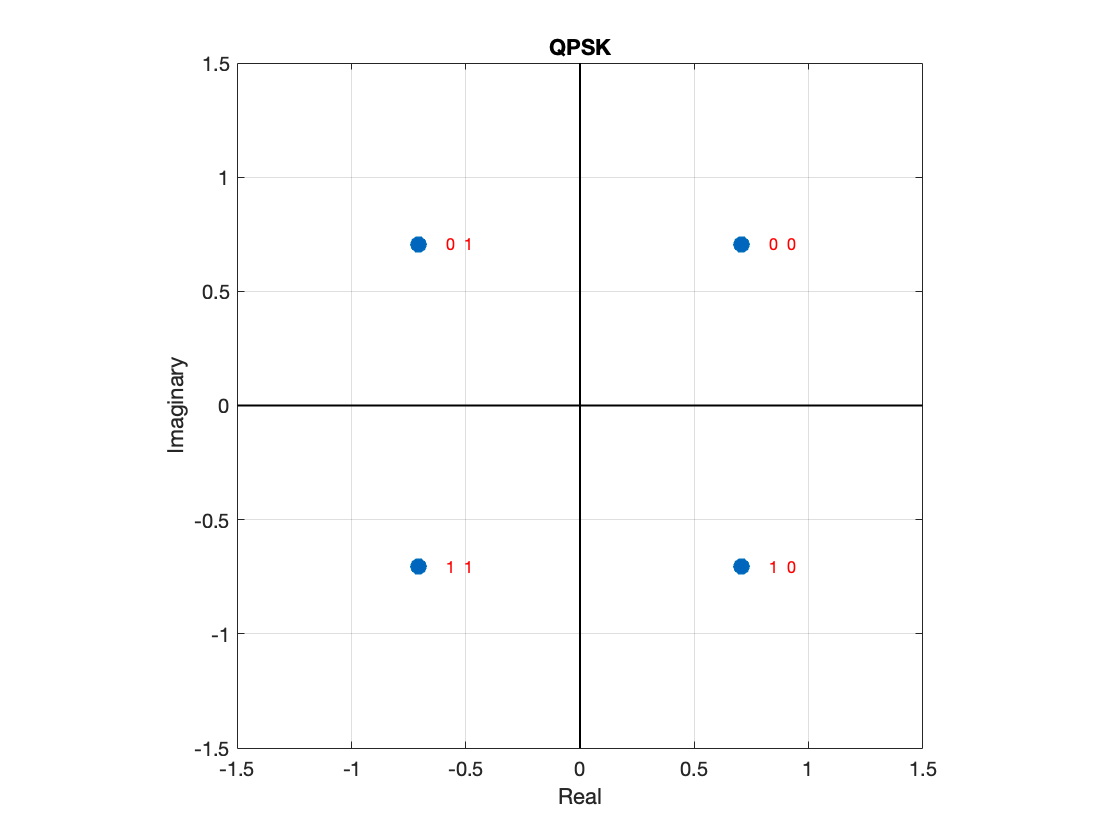
\includegraphics[width=0.6\textwidth]{Images/QPKS_Mapping.png}
  \caption{QPSK mapping.}
  \label{fig:QPKS_Mapping}
\end{figure}

The mapper groups the encoded bit stream into two-bit tuples $(b_1,b_0)$, converts each tuple to an integer index $(k =2b_1+b_0)$ and outputs \(s_k\).

The theoretical bit-error probability for QPSK in an AWGN channel is given by Equation \ref{eq:probErrQPSK}.
\begin{equation}
  P_b^{\text{QPSK}} = Q\left(\sqrt{2\frac{E_b}{N_0}}\right)
  \label{eq:probErrQPSK}
\end{equation}

\begin{figure}[h]
	\centering
	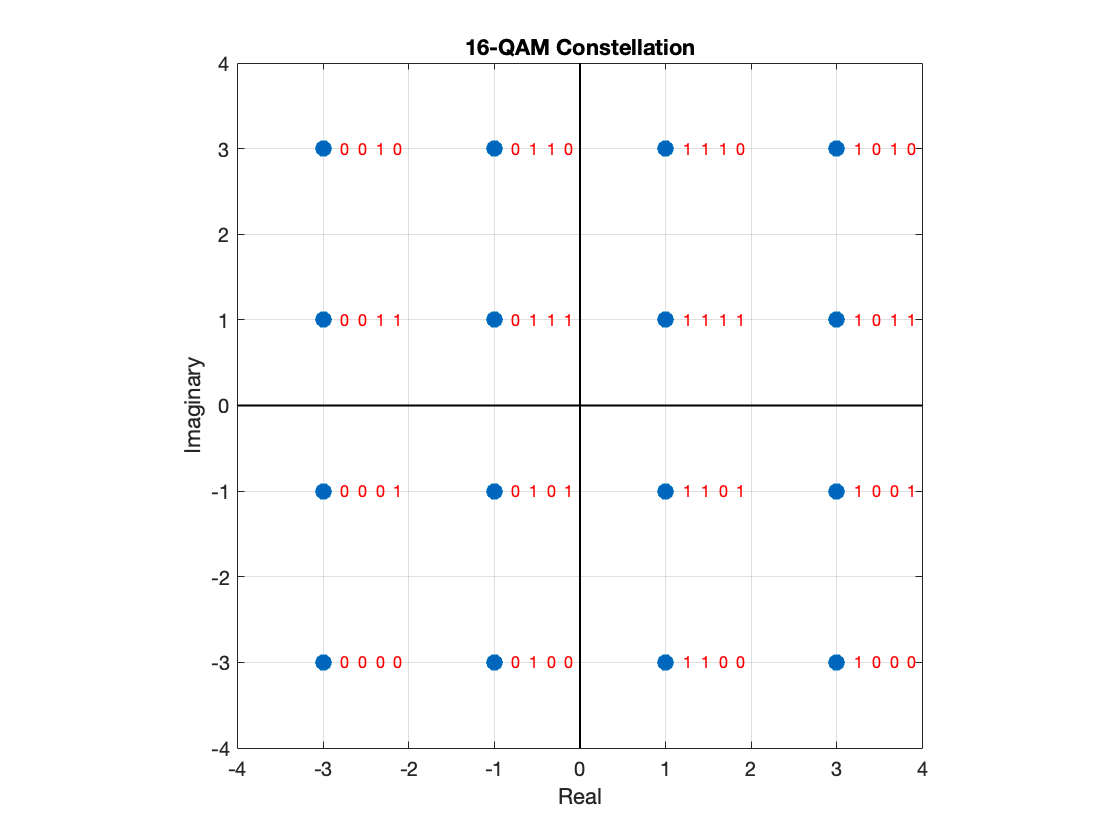
\includegraphics[width=0.6\textwidth]{Images/16-QAM_Constellation.png}
	\caption{16-QAM Gray mapping.}
	\label{fig:QAM_Mapping}
\end{figure}

A square $4\times4$ 16-QAM constellation is used. What changes comparing to the previous mapping approach is the fact that the amplitude also changes and for this specific mapping the phase and amplitude will not change consistently. The symbol position in the cartesian frame will be:
\[
I,R \in \{\pm3,\;\pm1\},\qquad
\]

The constellation points are labelled with \emph{Gray coding}, thus every nearest neighbour differs in \emph{exactly one} bit. Figure \ref{fig:QAM_Mapping}, shows how the codes are mapped.

Gray mapping was chosen because it minimises the bit‑error probability in an AWGN channel: a single symbol error (the most probable error event) flips only one bit, whereas natural or set‑partition labelling flips two or more bits on the same error~\cite{Work_TAC2025}.  

The theoretical bit-error probability for 16-QAM in an AWGN channel can be approximated by Equation \ref{eq:probErr16QAM}.

\begin{equation}
  
  P_b^{\text{16QAM}} \approx \frac{3}{4}Q\left(\sqrt{\frac{4}{5}\frac{E_b}{N_0}}\right)
  \label{eq:probErr16QAM}
\end{equation}

It is important to note that the QPSK and 16-QAM will have different bit energy, because they have different amplitudes. This will affect the SNR differently.


\subsection{Channel}

\label{sec:channel}

This section explains how the bit stream generated by the transmitter is carried through the physical channel in the simulator, how errors are detected at the receiver, and why the performance differs in an \textbf{AWGN} channel versus a \textbf{Rayleigh} fading channel.

The Channel block first converts the BitStream to a stream of symbols, then the FFT is computed, noise is added and the reverse is done, IFFT computed, and the symbols are decided and demodulated. Since the channel is perfectly synced there the time for the cyclic prefix is 0.

\subsubsection{AWGN}

For this channel transmitted symbols experience only additive noise—typically modeled as zero-mean white Gaussian noise. Because the noise affects all transmitted symbols uniformly, the bit-error rate (BER) depends mainly on the ratio between bit energy and noise density $E_b/N_{0}$. 

\subsubsection{Rayleigh}

Unlike AWGN, a Rayleigh channel models wireless environments where multiple paths cause random amplitude and phase fluctuations (flat fading). Each transmitted symbol is multiplied by a randomly varying complex channel gain with a Rayleigh-distributed amplitude. Some symbols experience deep fades with low instantaneous SNR, leading to bursts of bit errors. Thus, Rayleigh channels typically exhibit higher BER and a slower improvement as average SNR increases compared to AWGN. As a result, achieving very low error rates in Rayleigh fading typically demands stronger error-correction coding or additional diversity schemes.


